\RequirePackage[l2tabu,orthodox]{nag}  % warn about common LaTeX pitfalls
\RequirePackage[ascii]{inputenc}  % input is 7-bit ASCII
\RequirePackage{fixltx2e}  % fix LaTeX2e kernel bugs

\documentclass[11pt,twoside]{article}
\usepackage{color}
\usepackage{graphicx}
\graphicspath{ {image/} }
\usepackage{calc}  % arithmetic in length parameters
\usepackage{enumitem}  % more control over list formatting
\usepackage{fancyhdr}  % simpler headers and footers
\usepackage[margin=1in]{geometry}  % page layout
\usepackage{lastpage}  % for last page number
\usepackage{relsize}  % easier font size changes
\usepackage[normalem]{ulem}  % smarter underlining
\usepackage{url}  % verb-like typesetting of URLs
\usepackage{xfrac}  % nicer looking simple fractions for text and math
\usepackage{longtable}
\usepackage{tikz}
\usepackage{array}
\usepackage{tikz-timing}
\usetikzlibrary{arrows, shapes, backgrounds,fit}
\usepackage{tkz-graph}
% Set up fonts.
\usepackage[T1]{fontenc}  % use true 8-bit fonts
\usepackage{slantsc}  % allow slanted small-caps
\usepackage{microtype}  % perform various font optimizations
% Use Palatino-based monospace instead of kpfonts' default.
%\usepackage{newpxtext}
\ttfamily
\DeclareFontShape{T1}{\ttdefault}{m}{scsl}{<->ssub*\ttdefault/m/sc}{}
\DeclareFontShape{T1}{\ttdefault}{b}{scsl}{<->ssub*\ttdefault/b/sc}{}
% "Kepler" fonts.
\usepackage[nott,notextcomp]{kpfonts}
% Use curvier Latin Modern brackets instead of kpfonts' glyphs.
\DeclareSymbolFont{lmsymb}     {OMS}{lmsy}{m}{n}
\DeclareSymbolFont{lmlargesymb}{OMX}{lmex}{m}{n}
\DeclareMathDelimiter{\rbrace}{\mathclose}{lmsymb}{"67}{lmlargesymb}{"09}
\DeclareMathDelimiter{\lbrace}{\mathopen}{lmsymb}{"66}{lmlargesymb}{"08}

% Page layout: stretch text to fill up page.
\addtolength\footskip{.25\headheight}
\flushbottom

% Common list settings.

% Common macros.
\input{macros}
\newcommand*\st{\mathrel{|}}  % "such that" for set extension

% Headings.
\pagestyle{fancy}
\let\headrule\empty
\let\footrule\empty
\lhead{CSC\,418\,H1}
\chead{\large\scshape Assignment(b) \#\,2}
\rhead{\scshape Fall 2015}
\lfoot{\scshape Dept.\@ of Computer Science, University of Toronto,
       St.~George Campus}
\cfoot{}
\rfoot{\scshape page \thepage\space of \pageref{LastPage}}


\begin{document}

\begin{enumerate}[leftmargin=0pt]

\item  Drawing Penguin \\
Drawing penguin is basically like A1, we first creating some function which can draw cube, triangle prism and
trapezoidal prism. Using those functions to make different components.\\
\begin{itemize}
	\item $void \ drawCube()$ \\
         	Draw a unit cube
	\item $void \ TrapPrism()$ \\
 		draw a 3d trapezoidal prism with given length, width and height
	\item $void \ TriPrism()$\\
		draw triangle prism
\end{itemize}

 After done creating the shapes of all different components, let's start building the penguin. First draw the body in the middle of the window, then scale it. Then using translation takes us to local view relative to penguin's body then draw a component (i.e arm) give it some colour and scale it to a given size, then go back to world view(penguin's body)again and translation to another local view and draw another component. So every time we draw a component we always go to a local view relative penguin's body and after we done we go back to world view(penguin's body). Hence, when we moving penguin's body all other components are moving correspondingly. Especially, we need to notice that foot is also relatively to leg in the local view of leg, they are one component for world (penguin's body) but two separate parts if we go to the local view. This means when we moving leg, foot is moving correspondingly. And foot can also moving separately. Same for head, head also has subtrees, means when we moving head eye and mouth are also moving correspondingly. The structure tree below shows how does every part related to other parts and how does it move.
 \begin{center}
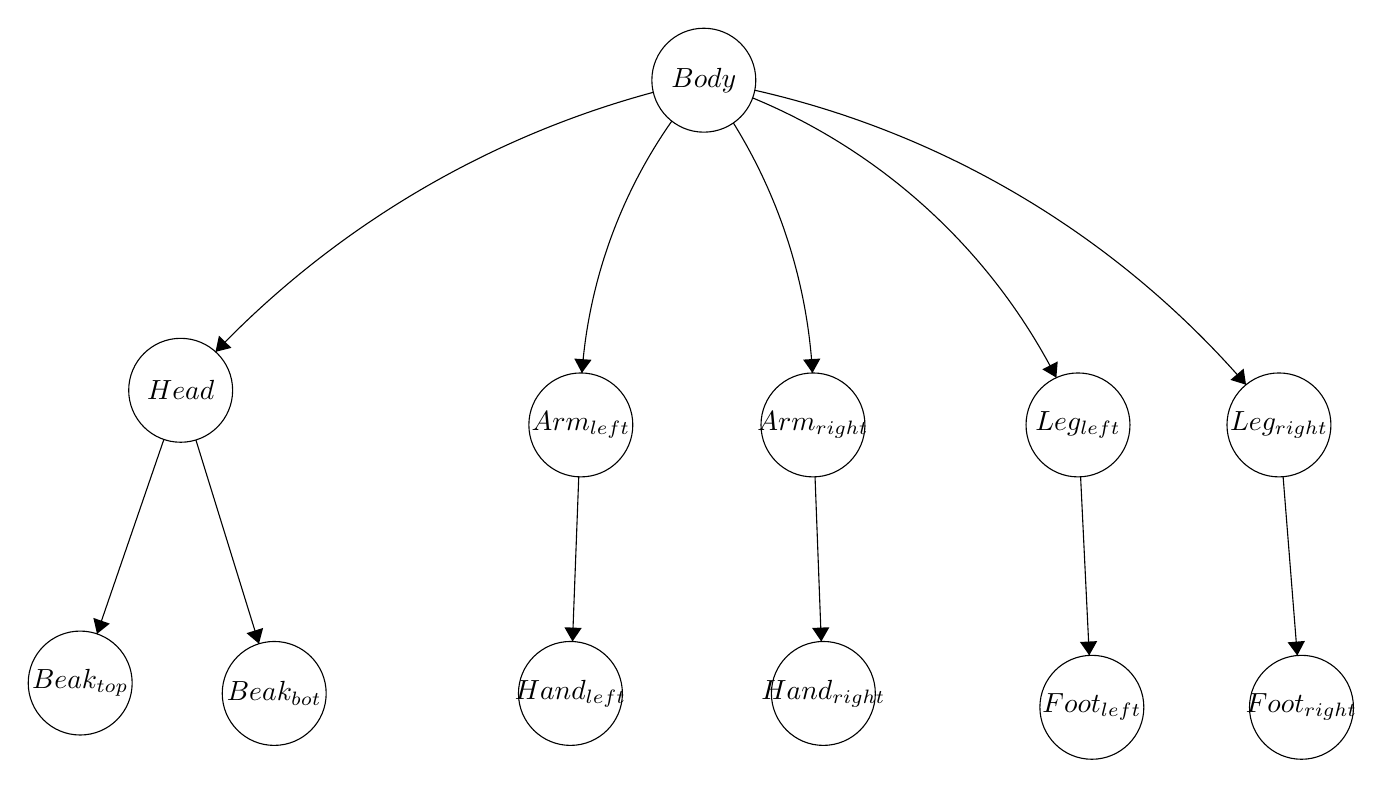
\begin{tikzpicture}[scale=0.22]
\tikzstyle{every node}+=[inner sep=0pt]
\draw [black] (40,-2.5) circle (3);
\draw (40,-2.5) node {$Body$};
\draw [black] (9.8,-20.4) circle (3);
\draw (9.8,-20.4) node {$Head$};
\draw [black] (32.9,-22.4) circle (3);
\draw (32.9,-22.4) node {$Arm_{left}$};
\draw [black] (46.3,-22.4) circle (3);
\draw (46.3,-22.4) node {$Arm_{right}$};
\draw [black] (61.6,-22.4) circle (3);
\draw (61.6,-22.4) node {$Leg_{left}$};
\draw [black] (4,-37.3) circle (3);
\draw (4,-37.3) node {$Beak_{top}$};
\draw [black] (15.2,-37.9) circle (3);
\draw (15.2,-37.9) node {$Beak_{bot}$};
\draw [black] (32.3,-37.9) circle (3);
\draw (32.3,-37.9) node {$Hand_{left}$};
\draw [black] (73.2,-22.4) circle (3);
\draw (73.2,-22.4) node {$Leg_{right}$};
\draw [black] (46.9,-37.9) circle (3);
\draw (46.9,-37.9) node {$Hand_{right}$};
\draw [black] (62.4,-38.7) circle (3);
\draw (62.4,-38.7) node {$Foot_{left}$};
\draw [black] (74.5,-38.7) circle (3);
\draw (74.5,-38.7) node {$Foot_{right}$};
\draw [black] (11.815,-18.178) arc (136.23101:105.08072:54.699);
\fill [black] (11.81,-18.18) -- (12.73,-17.95) -- (12.01,-17.25);
\draw [black] (8.83,-23.24) -- (4.97,-34.46);
\fill [black] (4.97,-34.46) -- (5.71,-33.87) -- (4.76,-33.54);
\draw [black] (10.68,-23.27) -- (14.32,-35.03);
\fill [black] (14.32,-35.03) -- (14.56,-34.12) -- (13.6,-34.42);
\draw [black] (32.964,-19.402) arc (-184.18828:-215.08288:28.981);
\fill [black] (32.96,-19.4) -- (33.52,-18.64) -- (32.52,-18.57);
\draw [black] (41.705,-4.967) arc (31.84462:3.28918:30.695);
\fill [black] (46.27,-19.4) -- (46.73,-18.57) -- (45.73,-18.63);
\draw [black] (42.819,-3.523) arc (67.55802:27.13347:34.495);
\fill [black] (60.35,-19.67) -- (60.43,-18.73) -- (59.54,-19.19);
\draw [black] (32.78,-25.4) -- (32.42,-34.9);
\fill [black] (32.42,-34.9) -- (32.95,-34.12) -- (31.95,-34.08);
\draw [black] (42.943,-3.08) arc (77.23334:40.88992:53.007);
\fill [black] (71.3,-20.08) -- (71.16,-19.15) -- (70.4,-19.8);
\draw [black] (46.42,-25.4) -- (46.78,-34.9);
\fill [black] (46.78,-34.9) -- (47.25,-34.08) -- (46.25,-34.12);
\draw [black] (61.75,-25.4) -- (62.25,-35.7);
\fill [black] (62.25,-35.7) -- (62.71,-34.88) -- (61.71,-34.93);
\draw [black] (73.44,-25.39) -- (74.26,-35.71);
\fill [black] (74.26,-35.71) -- (74.7,-34.87) -- (73.7,-34.95);
\end{tikzpicture}
\end{center}
\item Render Penguin\\
The penguin is rendered in a wireframe view.
\begin{itemize}
	\item $glPolygonMode( GL\_FRONT\_AND\_BACK, \  GL\_LINE ):$\\
         draw outlines of the penguin's shape
	\item  $glPolygonMode( GL\_FRONT\_AND\_BACK,\ GL\_FILL):$\\
	draw a solid view of penguin
\end{itemize}
Espcieally, for $solid \ with \ outline$ , we first draw the a solid view of penguin, and then call 
\[glEnable(GL\_POLYGON\_OFFSET\_LINE) \]
 After specifing the polygon offset, we can draw outlines on the top of solid view. \\
For Metallic and Matte, we needed to apply diffusion, ambience, specular and shiness
\[glMaterialfv \ \ \ \ \  glMaterialf\] 
 wereused to apply these properties for both metallic and matte renders.
\item Animation\\
Animation is created by keyframes of the penguin in different poses. Then using Catmull-Romm to interpolate those action to create animation.
\end{enumerate}

\end{document}